% Two tangent vectors v, w at a point p inside a coordinate patch c.
% Source: book/tex/diffgeo/forms.tex (§ Multivariable forms).
\documentclass[border=2mm]{standalone}
\usepackage{tikz}\usetikzlibrary{arrows.meta}\usepackage{amssymb}
\begin{document}
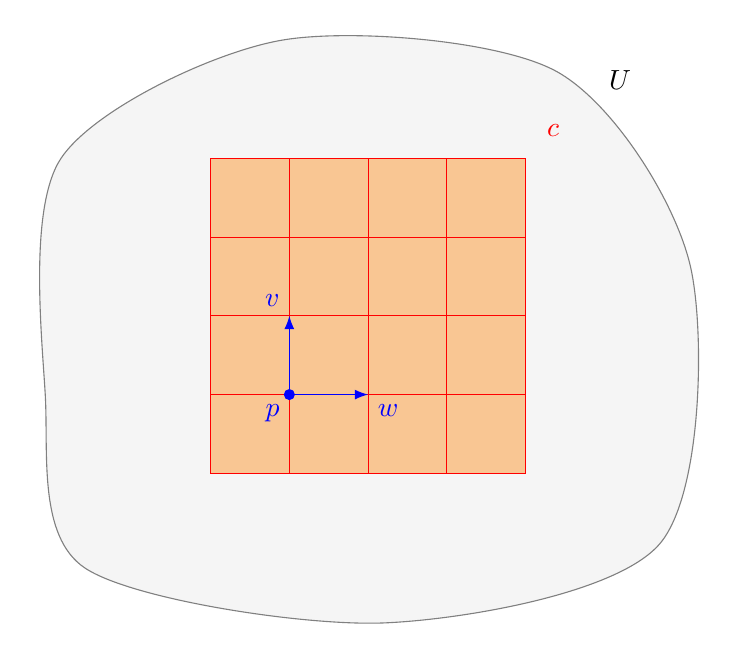
\begin{tikzpicture}
  \draw[gray,fill=gray!8] plot[smooth cycle] coordinates {(-3.6,-3.2)(0.2,-3.9)(3.7,-2.9)(4.1,0.6)(2.4,3.1)(-1.1,3.5)(-3.9,2)(-4.1,-1)}; \node at (3.2,3) {$U$};
  \fill[orange,opacity=0.4] (-2,-2) rectangle (2,2);
  \draw[red] (-2,-2) rectangle (2,2);
  \node[red] at (2.35,2.35) {$c$};
  \foreach \t in {-1,0,1}{\draw[red](-2,\t)--(2,\t);\draw[red](\t,-2)--(\t,2);}
  \fill[blue] (-1,-1) circle (2pt) node[below left,blue]{$p$};
  \draw[blue,-{Latex}] (-1,-1)--(-1,0) node[above left,blue]{$v$};
  \draw[blue,-{Latex}] (-1,-1)--(0,-1) node[below right,blue]{$w$};
\end{tikzpicture}
\end{document}
